\documentclass[xcolor=dvipsnames]{beamer}
\usepackage{amsmath}
\usepackage{hyperref}
\usepackage{ragged2e}
\usepackage{graphicx}
\usetheme{Copenhagen}
\usecolortheme[named=Black]{structure}

\title{BRIEF: Computing a Local Binary Descriptor Very Fast}
\author{Castleberry, Cherry, and Firth}
\renewcommand{\raggedright}{\leftskip=0pt \rightskip=0pt plus 0cm}

\begin{document}

\maketitle
\section{Introduction}
\subsection{Motivation}

\frame{\frametitle{Motivation: A 256-Byte Descriptor?}
 \begin{figure}
  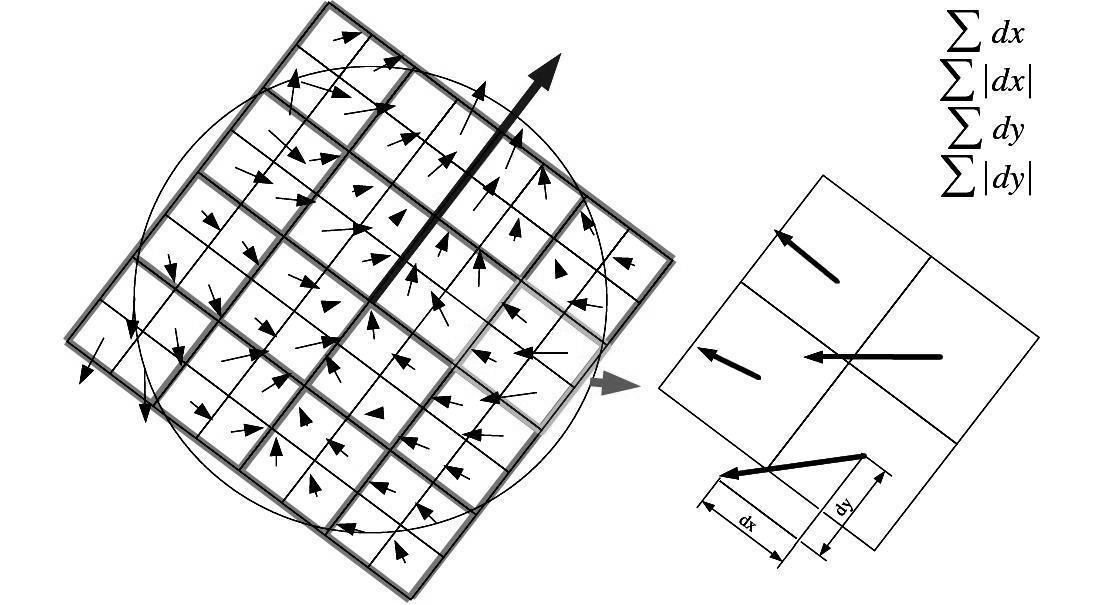
\includegraphics[width=\textwidth]{imgs/256-bytes.jpg}
  \caption{A SURF descriptor stores 64 orientation values as 4-byte integers.}
 \end{figure}
}

\subsection{Problem Definition}

\frame{\frametitle{Problem Definition: Make It Smaller, Compute It Faster}
 \setlength{\unitlength}{1mm}
 \begin{center}
 \begin{figure}
 \begin{picture}(30,30)
  \put(0,0 ){\circle*{5}} 
  \put(0,8 ){\circle*{5}} 
  \put(0,16){\circle*{5}} 
  \put(0,24){\circle*{5}} 
  \put(8,0 ){\circle*{5}} 
  \put(8,8 ){\circle*{5}} 
  \put(8,16){\circle*{5}} 
  \put(8,24){\circle*{5}} 
  \put(30,12){\circle*{5}} 
 \end{picture}
 \vspace{12pt}
 \caption{Reduce the size by a factor of 8.}
 \end{figure}
 \end{center}
}

\subsection{Previous Work}

\frame{\frametitle{Previous Work: Principal Component Analysis}
 \begin{figure}
  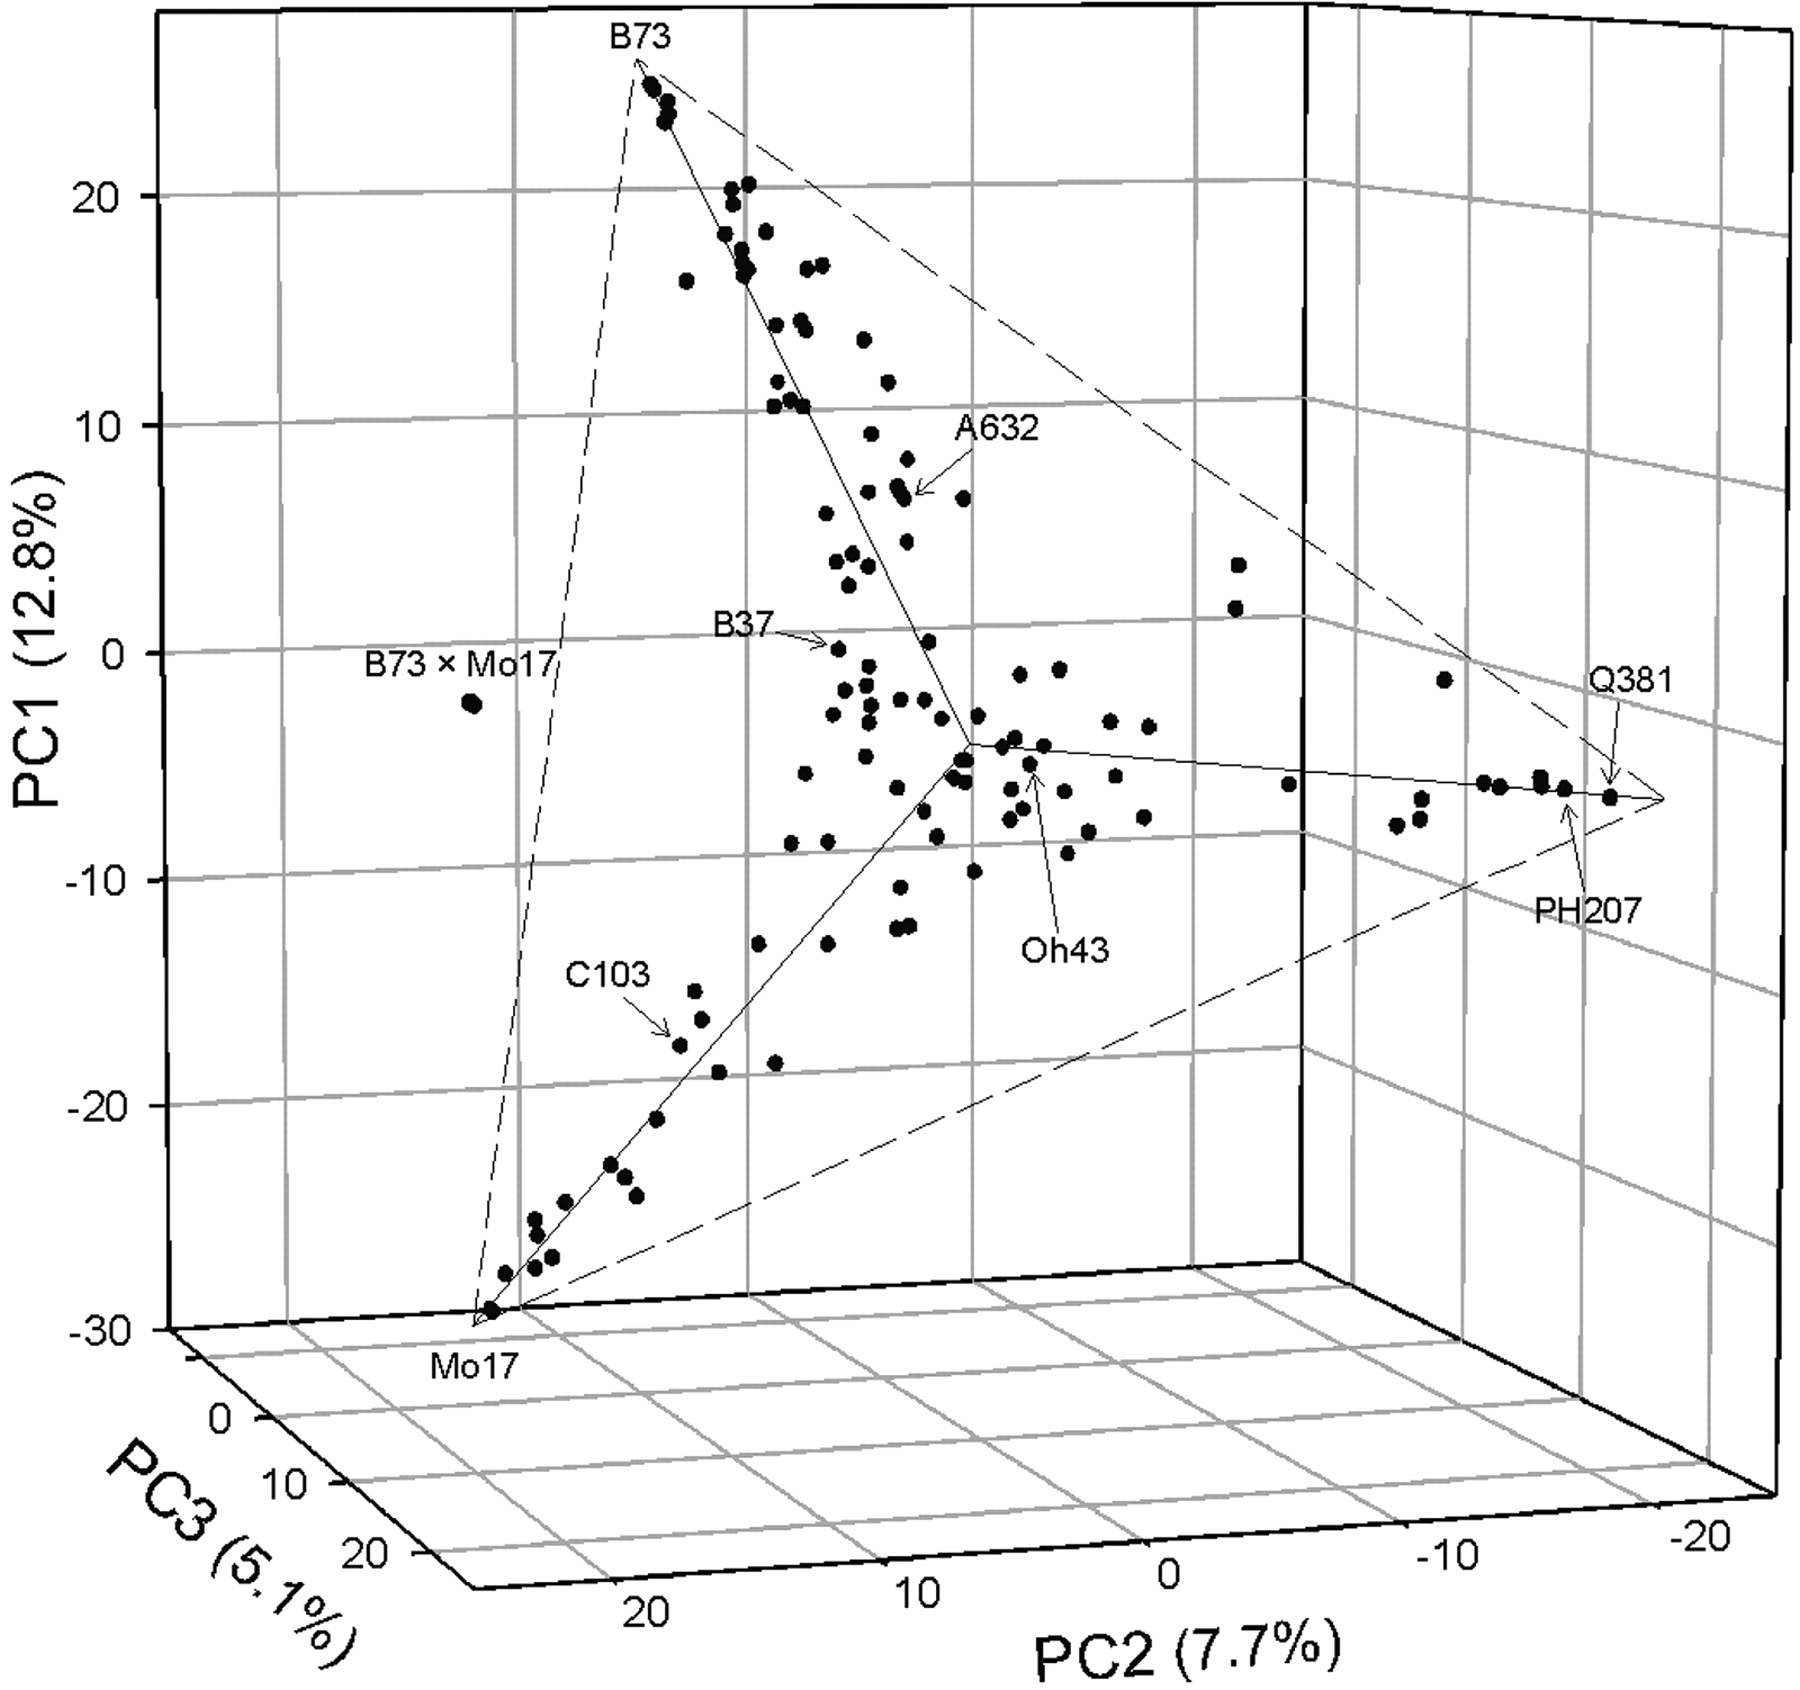
\includegraphics[width=.6\textwidth]{imgs/pca.jpg}
  \caption{PCA with Three Components.}
 \end{figure}
}

\frame{\frametitle{Previous Work: Floating-Point Quantization}
 \begin{figure}
  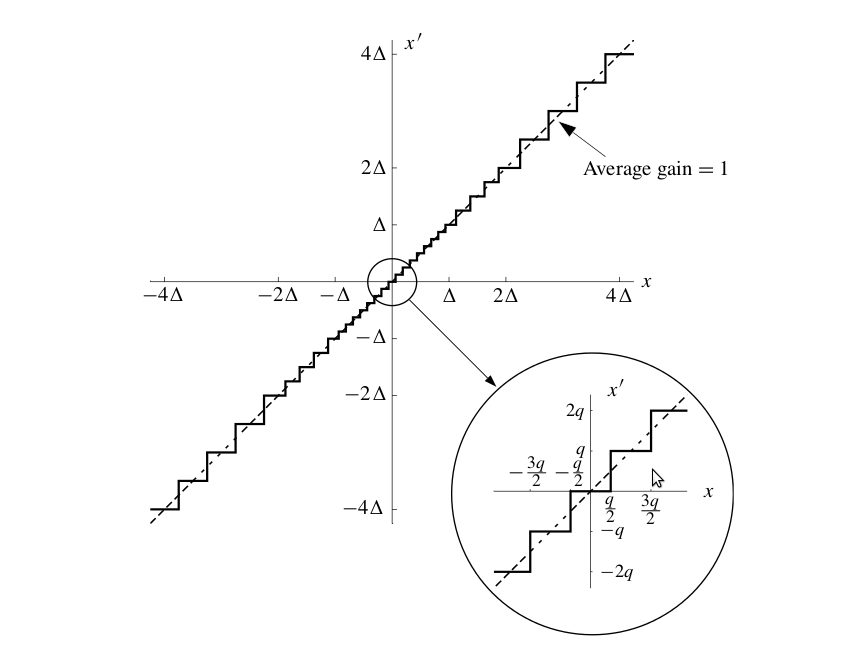
\includegraphics[width=.7\textwidth]{imgs/quantizer.png}
  \caption{Quantization with a 3-Bit Mantissa.}
 \end{figure}
}

\frame{\frametitle{Previous Work: Binarization}
 \begin{figure}
  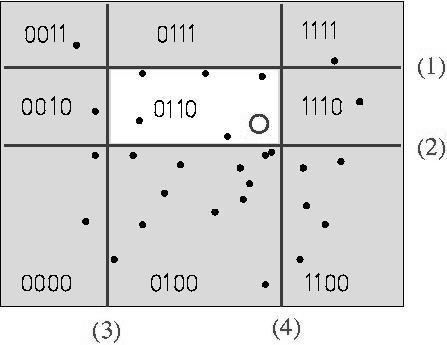
\includegraphics[width=.6\textwidth]{imgs/lsh.jpg}
  \caption{Locally Sentitive Hashing.}
 \end{figure}
}

\subsection{Background}
\section{Method}

\frame{\frametitle{Method: Patch Test}
 \begin{equation}
  \tau (p; \mathbf{x},y) :=
  \begin{Bmatrix}
   1 & \text{if}\ I(\mathbf{p},\mathbf{x}) < I(\mathbf{p},\mathbf{y}) \\
   0 & \text{otherwise}
  \end{Bmatrix}
 \end{equation}
}

\frame{\frametitle{Method: Descriptor Formula}
 \begin{equation}
  \sum_{I \leq i \leq n_d} 2^{i-1} \tau(p; x_i, y_i)
 \end{equation}
}

\subsection{Techniques Used}
\subsection{Method}
\subsection{Data}
\subsection{Experimental Setup}
\section{Conclusion}
\subsection{Results}
\subsection{Discussion}
\subsection{Conclusion}
\subsection{References}
\end{document}
